\chapter{Fundamentação teórica}\label{cap:background}

\section{Representação de Poses no espaço}

A representação de poses no espaço na robótica envolve o uso de sistemas de 
coordenadas, ou \emph{frames}, para descrever as posições e orientações de corpos 
rígidos, além das transformações entre esses frames. Um frame é composto por 
um ponto e um conjunto de vetores ortonormais que formam uma base do \(\mathbb{R}^3\). 
No contexto da robótica fixa, é comum especificar tarefas utilizando coordenadas 
cartesianas relativas a um frame de referência. Por exemplo, um ponto \(o_1^0\),
representando uma translação, pode ser expresso como um vetor com origem em um 
frame \(o_0 x_0 y_0 z_0\) e extremidade em outro frame \(o_1 x_1 y_1 z_1\), onde o expoente
indica em relação a qual frame as coordenadas são escritas. 
A orientação entre esses mesmos frames pode ser representada por uma matriz de rotação
\( R_1^0 \), pertencente ao grupo especial ortogonal de ordem 3 (\(SO(3)\)),
que possui a útil propriedade no cálculo da sua inversa: \((R_1^0)^{-1} = (R_1^0)^\top = R_0^1 \).

\begin{figure}
    \centering
    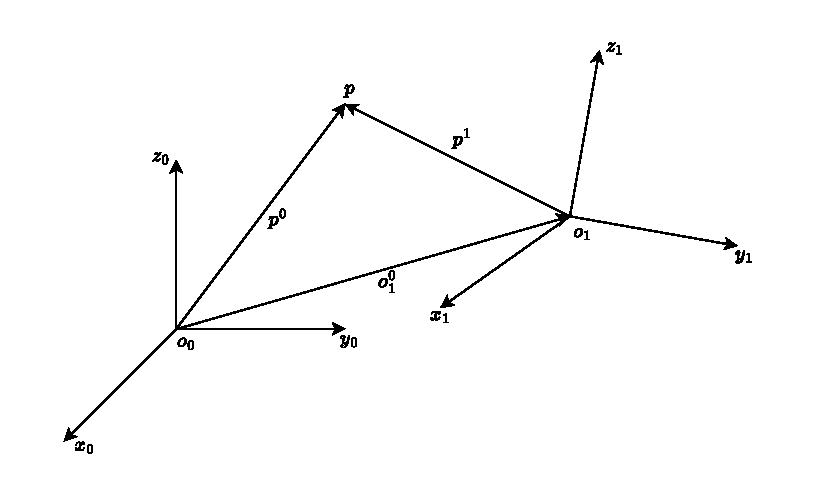
\includegraphics[width=0.8\linewidth]{Images/frames.pdf}
    \caption{Representação de um ponto \(p\) em diferentes frames.} \label{fig:frames}
\end{figure}

O grupo especial euclidiano de ordem 3 (\(SE(3)\)) combina rotações e 
translações em uma única representação, facilitando a descrição de 
deslocamentos rígidos no espaço tridimensional. Um deslocamento rígido 
é definido por um par ordenado \((R, d)\), onde \(R\) é uma matriz de 
rotação em \(SO(3)\) e \(d\) é um vetor de translação em \(\mathbb{R}^3\). Observando
a figura \ref{fig:frames}, podemos ver que a posição de um ponto \(p\) com relação
a um frame de referência \(o_0 x_0 y_0 z_0\) pode ser expressa como:

\begin{equation}\label{eq:rigid-motion}
    p^0 = R_1^0 p^1 + o_1^0
\end{equation}

Assim, a equação \ref{eq:rigid-motion} descreve um deslocamento rígido 
(rotação e translação) de um vetor fixado entre os dois frames.
Representando-a no formato matricial, utilizando coordenadas
homogêneas (com uma dimensão extra igual à unidade), teremos:

\begin{equation}
    \begin{bmatrix}
        p^0 \\
        1
    \end{bmatrix} = \begin{bmatrix}
        R_1^0 & o_1^0 \\
        0     & 1
    \end{bmatrix} \begin{bmatrix}
        p^1 \\
        1
    \end{bmatrix}
\end{equation}

ou numa notação mais compacta:

\begin{equation}
    \tilde{p^0} = T_1^0 \ \tilde{p^1}
\end{equation}

A matriz \(T_1^0\) de dimensão \(4 \times 4\) é denominada
\emph{matriz de transformação homogênea} e tem a característica
de que a sua inversa pode ser calculada através das componentes
de rotação e translação que compõe o deslocamento rígido:

\begin{equation}
    {(T_1^0)}^{-1} = \begin{bmatrix}
        R_1^0 & o_1^0 \\
        0     & 1
    \end{bmatrix}^{-1} = \begin{bmatrix}
        {(R_1^0)}^{\top} & -{(R_1^0)}^{\top} o_1^0 \\
        0                & 1
    \end{bmatrix}
\end{equation}

\section{Cinemática Direta}

Na robótica, uma cadeia cinemática é uma série de corpos rígidos conectados por 
juntas que permitem movimento relativo das partes móveis de um manipulador. 
Cadeias cinemáticas formam a base do estudo de manipuladores robóticos e geralmente 
são representadas por um grafo onde nós representam os elos e as arestas 
representam as juntas. Dependendo da topologia desse grafo, classifica-se 
uma cadeia cinemática de diferentes formas. Cadeias seriais do tipo aberta
são as mais comuns no âmbito de manipuladores robóticos utilizados 
em aplicações industriais. Nesses casos, seu grafo é representado por uma árvore 
onde cada nó possui apenas um único filho e o nó terminal da 
árvore usualmente representa o efetuador final (onde uma pinça ou garra robótica ficaria
acoplada, por exemplo).

As juntas prismáticas e de revolução são os tipos mais simples e introduzem um 
único grau de liberdade ao sistema. Juntas prismáticas permitem movimento 
translacional ao longo de uma direção, enquanto juntas de revolução possibilitam 
movimento rotacional ao redor de um eixo específico. Independentemente da 
complexidade das juntas, a maioria pode ser reduzida a uma combinação de juntas 
prismáticas e de revolução, facilitando a descrição das cadeias cinemáticas.

\begin{figure}
    \centering
    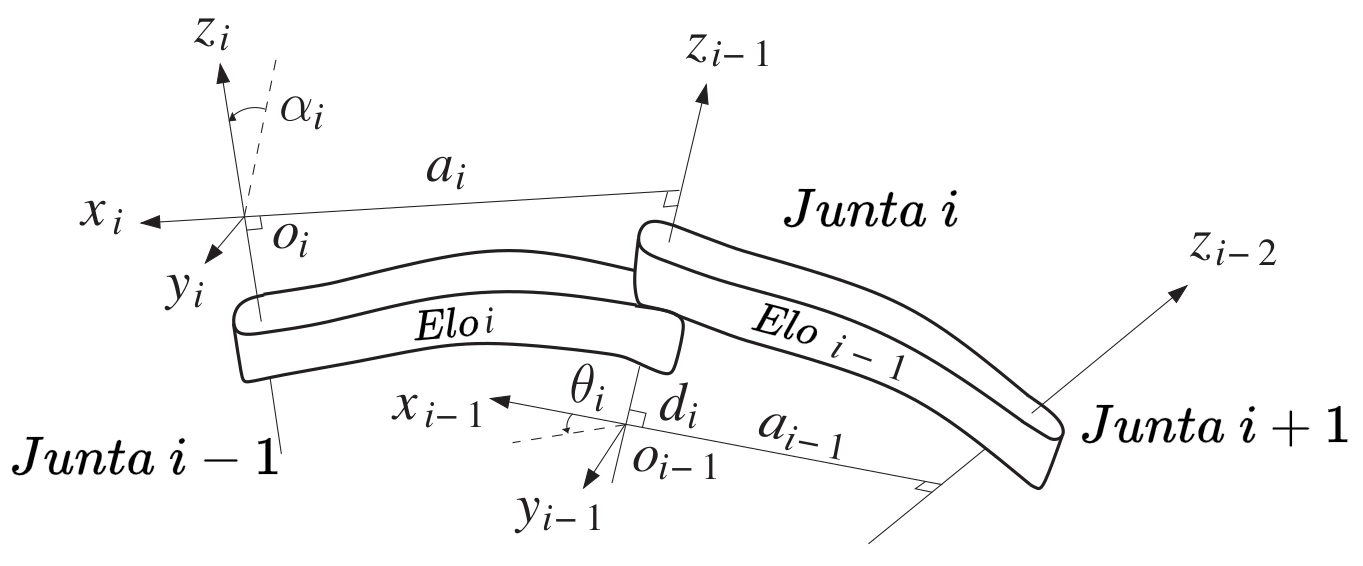
\includegraphics[width=0.8\linewidth]{Images/dh-assignment.png}
    \caption{Atribuição de \emph{frames} de acordo com a convenção de Denavit-Hartenberg. Adaptado de~\cite{spong_robot_2020}.}\label{fig:dh-assignment}
\end{figure}

Para calcular a cinemática direta, a cada elo \(i\) da cadeia é associado um frame 
\(o_i x_i y_i z_i\). Através da matriz de transformação homogênea \(A_i(q_i)\), expressa-se 
a pose de \(o_i x_i y_i z_i\) em relação a 
\(o_{i-1} x_{i-1} y_{i-1} z_{i-1}\). Para um manipulador com \(n\) juntas a sua configuração é dada pelo vetor \(q = [q_1 \ q_2 \ \ldots \ q_n]^\top\)
e a matriz de transformação homogênea \(T^0_n\) que fornece a pose
do efetuador final em relação ao frame da base é dada pela multiplicação matricial:

\begin{equation}\label{eq:fkine}
    T^0_n(q) = A_1(q_1) A_2(q_2) \cdots A_n(q_n) = \begin{bmatrix}
        R^0_n & o^0_n \\
        0     & 1
    \end{bmatrix}
\end{equation}

Apesar da colocação de frames em cada elo ser arbitrária, Jacques Denavit e Richard Hartenberg
introduziram uma convenção padronizada para fixação dos frames fornecendo uma representação mínima das transformações 
utilizando apenas 4 parâmetros~\cite{denavit1955}: ângulo da junta  (\(\theta_i\)), deslocamento do elo (\(d_i\)), comprimento do elo (\(a_i\)) e 
torção do elo (\(\alpha_i\)). A figura~\ref{fig:dh-assignment} ilustra a relação entre dois \emph{frames} de uma cadeia cinemática que segue tal convenção, 
fornecendo uma interpretação geométrica de cada parâmetro.

\begin{align}~\label{eq:dh-matrix}
    A_i & = Rot_z(\theta_i) \cdot Trans_z(d_i) \cdot Trans_x(a_i) \cdot Rot_x(\alpha_i)             
\end{align}

Tal representação mínima só é possível devido a introdução de 
duas restrições na colocação dos frames em cada elo~\cite{spong_robot_2020}:

\begin{itemize}
    \item (\textbf{DH1}) $x_i$ intersecta o eixo $z_{i-1}$
    \item (\textbf{DH2}) $x_i$ é perpendicular o eixo $z_{i-1}$
\end{itemize}

A tabela~\ref{tab:dh-parameters} descreve de maneira detalhada
a definição de cada parâmetro na \emph{convenção Denavit-Hartenberg} (DH).

\begin{table}[htbp]
    \centering
    \begin{tabular}{c c}
        \toprule
        \textbf{Parâmetro} & \textbf{Definição}                                                                                             \\
        \midrule
        $\theta_i$         & \makecell[l]{O ângulo entre os eixos $\mathbf{x}_{i-1}$ e $\mathbf{x}_i$ em torno do eixo $\mathbf{z}_{i-1}$}  \\
        \midrule
        $d_i$              & \makecell[l]{A distância da origem do sistema de coordenadas $\{i-1\}$                                         \\ até o eixo $\mathbf{x}_i$ ao longo do eixo $\mathbf{z}_{i-1}$} \\
        \midrule
        $a_i$              & \makecell[l]{A distância entre os eixos $\mathbf{z}_{i-1}$ e $\mathbf{z}_i$ ao longo do eixo $\mathbf{x}_i$;   \\ para eixos que se intersectam, é paralela a $\mathbf{z}_{i-1} \times \mathbf{z}_i$} \\
        \midrule
        $\alpha_i$         & \makecell[l]{O ângulo entre o eixo $\mathbf{z}_{i-1}$ e o eixo $\mathbf{z}_i$ em torno do eixo $\mathbf{x}_i$} \\
        \bottomrule
    \end{tabular}
    \caption{Descrição dos parâmetros Denavit-Hartenberg}\label{tab:dh-parameters}
\end{table}

\subsection{Cinemática direta de um braço planar}

Um braço planar é um tipo de manipulador serial cujo espaço de trabalho se
limita a um plano. A figura~\ref{fig:3r-planar-arm} mostra um braço planar do
tipo 3R, o qual possui três elos e três juntas de revolução acoplados em série.
A escolha da colocação do frame da base \(o_0x_0y_0z_0\) é totalmente
arbitrária e ao tomar como indicado na figura (com o eixo \(z\) apontando para
fora do papel) a fixação dos frames subsequentes na cadeia cinemática fica
restrita a convenção de Denavit-Hartenberg adotada. A tabela DH para esse
manipulador é dada por:

\begin{table}[htbp]
    \centering
    \begin{tabular}{c c c c c}
        \toprule
        \textbf{Elo} & \(\theta\)   & \(d\) & \(a\)   & \(\alpha\) \\
        \midrule
        1            & \(\theta_1\) & 0     & \(a_1\) & 0          \\
        2            & \(\theta_2\) & 0     & \(a_2\) & 0          \\
        3            & \(\theta_3\) & 0     & \(a_3\) & 0          \\
        \bottomrule
    \end{tabular}
    \caption{Parâmetros DH para o braço planar 3R da figura~\ref{fig:3r-planar-arm}.}\label{tab:dh-parameters-planar-arm}
\end{table}

Dados os valores fixos \(a_i\) que indicam o comprimento do elo \(i\), as
únicas variáveis livres no cálculo da cinemática direta são os ângulos das
juntas ($q_i = \theta_i$). Para \(i = 1, 2, 3\) as matrizes $A_i$ são calculadas 
com o auxílio da equação~\ref{eq:dh-matrix}:

\begin{figure}
    \centering
    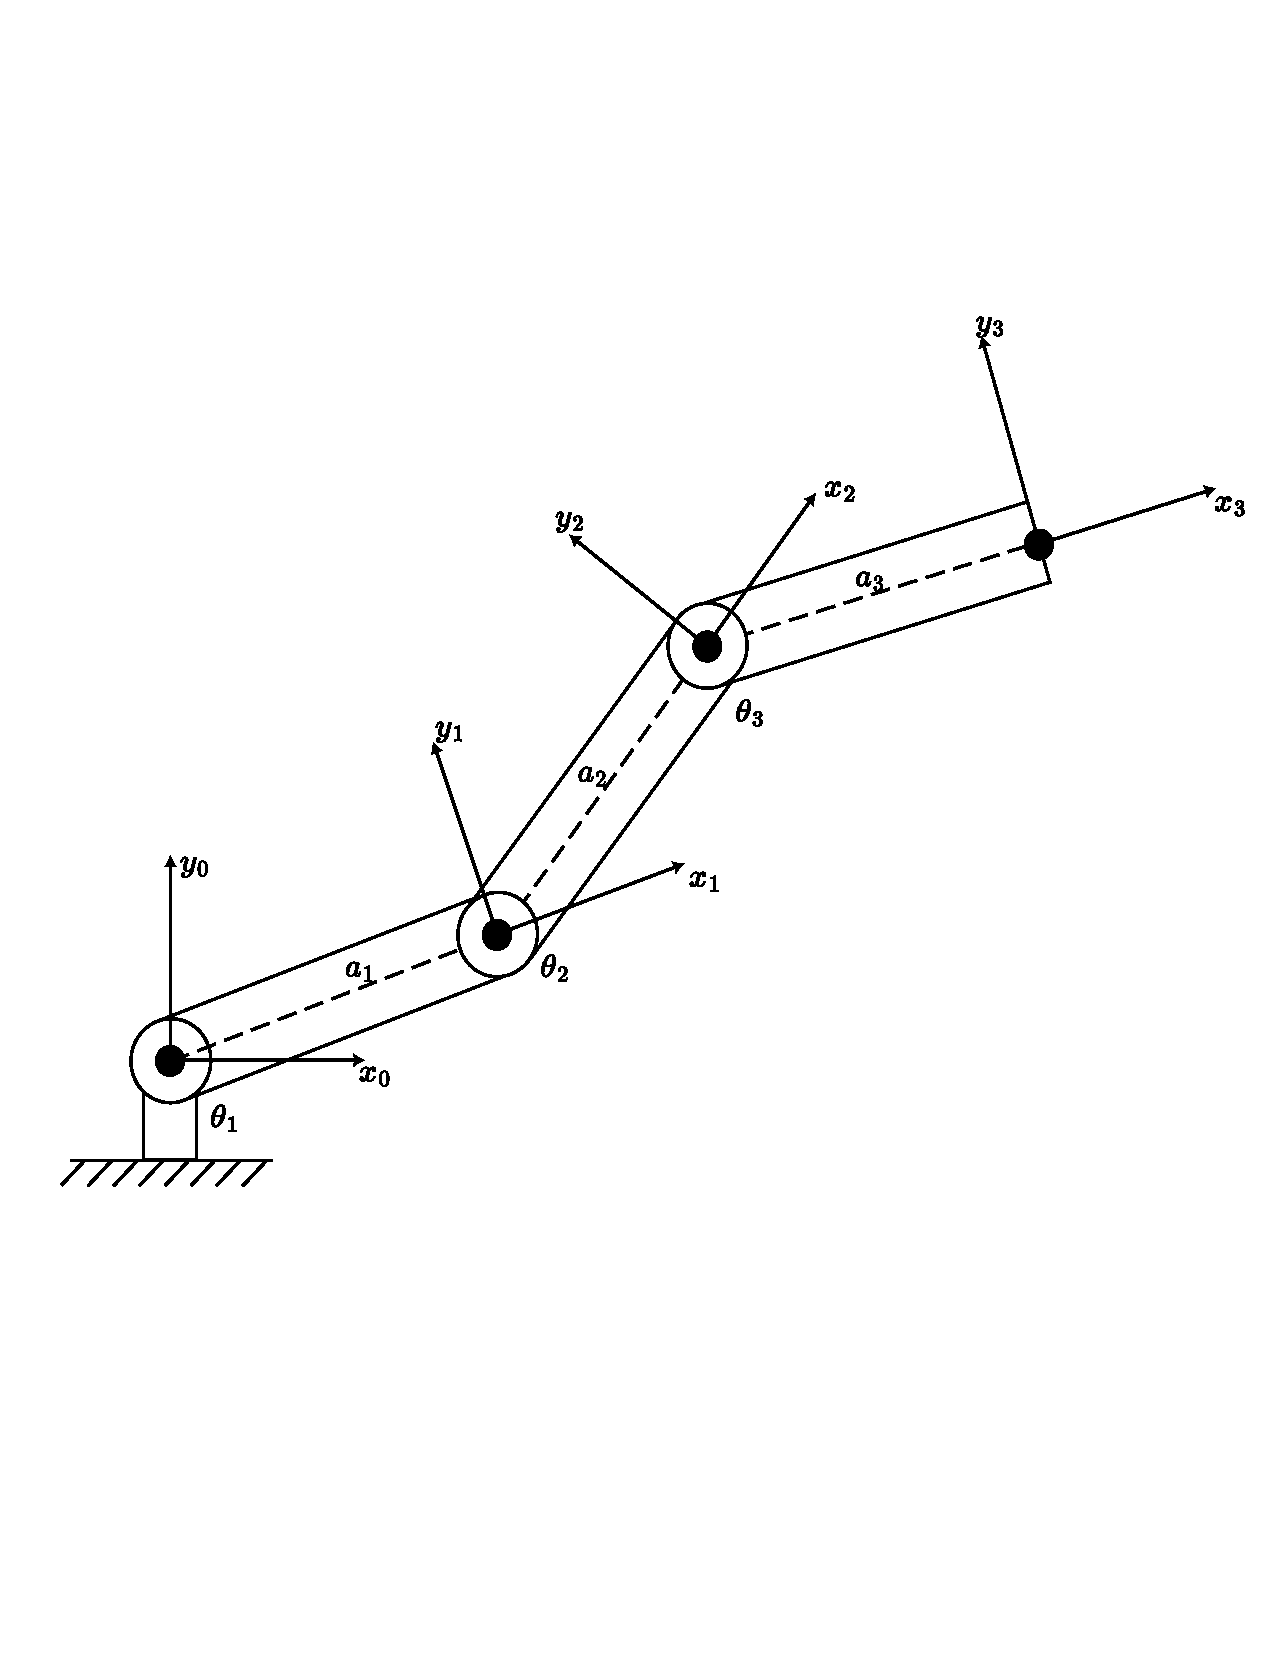
\includegraphics[width=0.8\linewidth]{Images/3r-planar.pdf}
    \caption{Braço planar do tipo 3R.}\label{fig:3r-planar-arm}
\end{figure}

\begin{equation}
    \mathbf{A}_i = \begin{bmatrix}
        c_i & -s_i & 0 & a_i c_i \\
        s_i & c_i  & 0 & a_i s_i \\
        0   & 0    & 1 & 0       \\
        0   & 0    & 0 & 1
    \end{bmatrix}
\end{equation}

onde \(\theta_1 + \theta_2 = \theta_{12}\), \(\cos(\theta_1 + \theta_2) = c_{12}\) e assim por diante. 

Já para as matrizes \(T^0_i\), utiliza-se a equação~\ref{eq:fkine}:

\begin{equation}
    \mathbf{T}^0_1 = \mathbf{A}_1
\end{equation}

\begin{equation}
    \mathbf{T}^0_2 = \mathbf{A}_1 \cdot \mathbf{A}_2 = \begin{bmatrix}
        c_{12} & -s_{12} & 0 & a_1c_1 + a_2c_{12} \\
        s_{12} & c_{12}  & 0 & a_1s_1 + a_2s_{12} \\
        0      & 0       & 1 & 0                  \\
        0      & 0       & 0 & 1
    \end{bmatrix}
\end{equation}

\begin{equation}
    \mathbf{T}^0_3 = \mathbf{A}_1 \cdot \mathbf{A}_2 \cdot \mathbf{A}_3 = \begin{bmatrix}
        c_{123} & -s_{123} & 0 & a_1c_1 + a_2c_{12} + a_3c_{123} \\
        s_{123} & c_{123}  & 0 & a_1s_1 + a_2s_{12} + a_3s_{123} \\
        0       & 0        & 1 & 0                               \\
        0       & 0        & 0 & 1
    \end{bmatrix}
\end{equation}

As três primeiras entradas da última coluna da matriz \(T^0_3\) dão a posição
\(\mathbf{P} = {\left[ x \ y \ z \right]}^{\top}\) do efetuador final em função
da configuração do manipulador. Note que $z = 0$ quaisquer que sejam os ângulos
das juntas pois, como esperado, o manipulador é planar. Além disso, analisando
a componente de rotação, fica evidente que a orientação do efetuador final com
relação ao frame da base é dada pela soma dos ângulos das juntas: $\psi =
    \theta_{123}$.

\section{Cinemática Diferencial}

Na seção anterior foi apresentado como podemos estabelecer uma relação entre a
configuração de um manipulador com $n$ juntas e a pose do efetuador final no
espaço SE3. Esta seção introduz o conceito da matriz jacobiana do manipulador,
responsável por estabelecer um mapeamento linear entre um vetor de velocidades no espaço
 das juntas com a velocidade do efetuador no espaço de trabalho. A seção termina analisando o 
problema da cinemática inversa diferencial o qual proporciona a execução de trajetórias 
cartesianas, no espaço de trabalho do manipulador.

\subsection{A Jacobiana do Manipulador}

Dado um manipulador com $n$ juntas vamos considerar

\begin{equation}
    T_{n}^{0}(q) = \begin{bmatrix}
        R_{n}^{0}(q) & o_{n}^{0}(q) \\
        0            & 1
    \end{bmatrix}
\end{equation}

a transformação homogênea que expressa a pose do efetuador final com relação ao
\emph{frame} da base que, como já vimos, é função apenas da configuração \(q =
\begin{bmatrix}
    q_1 & \cdots & q_n
\end{bmatrix}^\top\).

As relações entre as componentes da velocidade do efetuador final
são estabelecidas da seguinte forma:

\begin{align}
    v_n^0 = J_v \dot{q} \\
    \omega_n^0 = J_\omega \dot{q}
\end{align}

onde \(v_n^0\) e \(\omega_n^0\) expressam respectivamente as velocidades linear
e angular do efetuador final e \(J_v\), \(J_\omega\) são matrizes de dimensão
\(3 \times n\). De maneira mais compacta, pode-se escrever

\begin{equation}
    \xi = J \dot{q}
\end{equation}

onde teremos:

\begin{equation}
    \xi = \begin{bmatrix}
        v_n^0 \\
        \omega_n^0
    \end{bmatrix} \text{ e } J = \begin{bmatrix}
        J_v \\
        J_\omega
    \end{bmatrix}
\end{equation}

O vetor \(\xi\) de dimensão \(6 \times 1\) é denominado de velocidade do corpo
rígido (em inglês \emph{body velocity} ou \emph{twist}). Note também que a
matriz \(J\), chamada \emph{jacobiana do manipulador} ou simplesmente
jacobiana, é usualmente uma matriz de dimensão \(6 \times n\).

A parte superior da matriz jacobiana \(J_v\) será:

\begin{equation}
    J_v = \begin{bmatrix}
        J_{v_1} & J_{v_2} & \cdots & J_{v_n}
    \end{bmatrix}
\end{equation}

onde a i-ésima coluna \(J_{v_i}\) é dada por:

\begin{equation}
    J_{v_i} =
    \begin{cases}
        z_{i-1}^0 \times (o_n^0 - o_{i-1}^0) & \text{se a junta $i$ é de revolução} \\
        z_{i-1}                              & \text{se a junta $i$ é prismática}   \\
    \end{cases}
\end{equation}

Já a parte inferior da matriz jacobiana \(J_\omega\) será:

\begin{equation}
    J_\omega = \begin{bmatrix}
        J_{\omega_1} & J_{\omega_2} & \cdots & J_{\omega_n}
    \end{bmatrix}
\end{equation}

onde a i-ésima coluna \(J_{\omega_i}\) é dada por:

\begin{equation}
    J_{\omega_i} =
    \begin{cases}
        z_{i-1}^0 & \text{se a junta $i$ é de revolução} \\
        0         & \text{se a junta $i$ é prismática}   \\
    \end{cases}
\end{equation}

Note que o cálculo da jacobiana torna-se possível apenas com o conhecimento da
função de cinemática direta \(T_n^0\) mostrando-se uma maneira eficiente para calcular 
não so a velocidade do efetuador final mas também a velocidade de qualquer ponto da 
estrutura cinemática do manipulador.

Como exemplo, considere o manipulador planar 3R introduzido na seção anterior.
Com base no procedimento descrito acima, a jacobiana do manipulador é dada por:

\begin{equation}
    J(q) = \begin{bmatrix}
        z_0^0 \times (o_3^0 - o_0^0) & z_1^0 \times (o_3^0 - o_1^0) & z_2^0 \times (o_3^0 - o_2^0) \\
        z_0^0                        & z_1^0                        & z_2^0
    \end{bmatrix}
\end{equation}

onde as termos envolvidos são:

\begin{align*}
    o_0^0 = \begin{bmatrix}
                0 \\
                0 \\
                0
            \end{bmatrix} \ \ o_1^0 = \begin{bmatrix}
                                          a_1 c_1 \\
                                          a_1 s_1 \\
                                          0
                                      \end{bmatrix} \ \ o_2^0 & = \begin{bmatrix}
                                                                      a_1 c_1 + a_2 c_{12} \\
                                                                      a_1 s_1 + a_2 s_{12} \\
                                                                      0
                                                                  \end{bmatrix} \ \ o_3^0 = \begin{bmatrix}
                                                                                                a_1 c_1 + a_2 c_{12} + a_3 c_{123} \\
                                                                                                a_1 s_1 + a_2 s_{12} + a_3 s_{123} \\
                                                                                                0
                                                                                            \end{bmatrix} \\
    z_0^0                                     & = z_1^0 = z_2^0 = \begin{bmatrix}
                                                                      0 \\
                                                                      0 \\
                                                                      1
                                                                  \end{bmatrix}
\end{align*}

Desenvolvendo as expressões acima, obtém-se:

\begin{equation}
    J(q) = \begin{bmatrix}
        -a_1 s_1 - a_2 s_{12} - a_3 s_{123} & -a_2 s_{12} - a_3 s_{123} & -a_3 s_{123} \\
        a_1 c_1 + a_2 c_{12} + a_3 c_{123}  & a_2 c_{12} + a_3 c_{123}  & a_3 c_{123}  \\
        0                                   & 0                         & 0            \\
        0                                   & 0                         & 0            \\
        0                                   & 0                         & 0            \\
        1                                   & 1                         & 1            \\
    \end{bmatrix}
\end{equation}

Note que o manipulador planar não provoca qualquer translação ao longo do eixo
\(z\) uma vez que qualquer contribuição de \(J_{v_i}\) é nula na terceira
componente. Além disso, a única componente de rotação influenciada pelo
movimento das juntas é a rotação em torno também do eixo do eixo \(z\)
evidenciado pela terceira componente de \(J_{\omega_i}\) igual a 1.

\subsection{Singularidades}

A matriz jacobiana, de dimensão \(6 \times n\), estabelece o mapeamento linear
entre as velocidades das juntas e do efetuador final através da relação:

\begin{equation}\label{eq:jacobian-mapping}
    \xi = J(q) \dot{q}
\end{equation}

que coloca de forma explícita a dependência da configuração atual do
manipulador no cálculo de \(J\). Tal mapeamento implica que qualquer vetor de
velocidades do efetuador final é uma combinação linear das colunas da matriz
jacobiana:

\begin{equation}
    \xi = J_1 \dot{q_1} + J_2 \dot{q_2} + \cdots + J_n \dot{q_n}
\end{equation}

Uma vez que \(\xi \in \mathbb{R}^6\) o manipulador so conseguirá desempenhar
uma velocidade arbitrária se todas as colunas de \(J\) forem linearmente
independentes, ou seja, quando o posto da matriz jacobiana for igual a \(6\).
Para uma matriz \(J \in \mathbb{R}^{6 \times n}\) é sempre verdade que
\(\text{posto}(J) \leq \min(6, n)\). Com efeito, no caso do manipulador planar
3R têm-se \(n = 3\) e desse modo \(\text{posto}(J) \leq 3\) evidenciando o
fato de que o manipulador não consegue desenvolver qualquer velocidade no
espaço de trabalho.

Configurações paras as quais o posto da matriz jacobiana é menor que o máximo
possível (em inglês \emph{rank deficiency}) são denominadas de
\emph{singularidades} ou configurações singulares. Identificar configurações
singulares é de grande importância para o controle de manipuladores por
diversos motivos, entre eles~\cite{spong_robot_2020}:

\begin{itemize}
    \item Singularidades representam configurações nas quais a mobilidade do manipulador
          é reduzida, ou seja, não é possível impor um movimento arbitrário ao efetuador
          final.
    \item Quando o manipulador está em uma singularidade, pode haver infinitas soluções
          para o problema de cinemática inversa.
    \item Nas proximidades de uma singularidade, pequenas variações nas velocidades no
          espaço operacional podem causar velocidades ilimitadas no espaço das juntas.
\end{itemize}

Quando a matriz jacobiana é quadrada, podemos usar o fato de que seu
determinante se anula em configurações singulares, contudo ainda assim o
problema de determinar o conjunto de configurações é difícil, uma vez que é necessário
resolver a equação

\begin{equation}
    \det(J(q)) = 0
\end{equation}

que geralmente envolve termos com alto grau de não linearidade. Nas próximas
seções, serão examinadas técnicas que viabilizam um esquema de controle capaz de se
afastar de configurações singulares ao explorar a redundância presente em
manipuladores planares. Isso se refere a casos em que a matriz Jacobiana é
retangular, apresentando mais velocidades no espaço das juntas (colunas) do que
velocidades possíveis no espaço de trabalho (linhas).

\subsection{Cinemática Inversa Diferencial}

Se a matriz jacobiana definida na equação (\ref{eq:jacobian-mapping}) é
quadrada e não singular, o problema de cinemática inversa pode ser resolvido
através da simples inversão da mesma:

\begin{equation}\label{eq:resolved-rate}
    \dot{q} = J^{-1}(q) \xi
\end{equation}

Se a configuração inicial do manipulador \(q(0)\) é conhecida, as posições das
juntas podem ser calculadas integrando as velocidades no tempo:

\begin{equation}
    q(t) = q(0) + \int_{0}^{t} \dot{q}(\tau) d\tau
\end{equation}

A integração em tempo discreto pode ser feita utilizando técnicas de métodos
numéricos. A abordagem mais simples consiste na integração pelo método de
Euler, onde as posições das juntas no instante atual \(t_k\) são utilizadas
para calcular a configuração do manipulador no instante posterior \(t_{k+1} =
t_k + \Delta t\):

\begin{align}
    q(t_{k + 1}) & = q(t_k) + \dot{q}(t_k) \delta_t
\end{align}

onde \(\delta_t\) é um intervalo de integração apropriado (tempo de
amostragem).

O esquema de controle descrito acima é conhecido como \emph{
    Resolved Rate Motion Control} (RRMC), o qual consegue de 
maneira simples e elegante o solucionar o problema de gerar movimentos no efetuador 
final de velocidade constante sem recorrer à soluções numéricas ou analíticas para 
o cálculo da cinemática inversa~\cite{corke_robotics_2023}. 
Tal esquema é útil na geração de trajetórias contínuas e suaves no espaço de trabalho,
conhecidas como trajetórias cartesianas.

Como exemplo, ainda considerando o manipulador planar 3R, ao especificar apenas
um vetor de velocidades \(\xi\) que leva em conta as componentes do
plano \(xy\) da velocidade linear e a componente de rotação angular em torno do
eixo \(z\), têm-se que:

\begin{equation}
    \xi = \begin{bmatrix}
        v_x \\
        v_y \\
        \omega_z
    \end{bmatrix}
\end{equation}

Assim a matriz jacobiana se torna livre das linhas que possuem apenas zeros:

\begin{equation}
    J(q) = \begin{bmatrix}
        -a_1 s_1 - a_2 s_{12} - a_3 s_{123} & -a_2 s_{12} - a_3 s_{123} & -a_3 s_{123} \\
        a_1 c_1 + a_2 c_{12} + a_3 c_{123}  & a_2 c_{12} + a_3 c_{123}  & a_3 c_{123}  \\
        1                                   & 1                         & 1
    \end{bmatrix}
\end{equation}

e contanto que não seja singular pode ser facilmente invertida. Como exemplo, para gerar 
um movimento retilíneo no efetuador final paralelo
ao eixo \(x\) do plano \(xy\) com velocidade constante, basta tomar \(\xi = \begin{bmatrix}
    v_x & 0 & 0
\end{bmatrix}^\top\).

\section{Manipuladores redundantes}

Manipuladores cinematicamente redundantes, são aqueles que possuem mais juntas
do que o número estritamente necessário para a execução de uma determinada
tarefa. Este excedente de juntas confere a esses manipuladores um nível
aumentado de destreza, permitindo-lhes navegar em ambientes complexos com maior
flexibilidade. Esta seção introduz uma solução geral para o problema
da cinemática inversa diferencial quando a matriz jacobiana é retangular,
envolvendo o conceito da sua \emph{pseudo-inversa}. Em seguida, utilizando a
decomposição em valores singulares de \(J\) obtém-se uma descrição
geométrica e qualitativa da destreza associada à uma dada configuração através
dos conceitos do elipsoide e da medida de manipulabilidade. Ao final da seção,
utiliza-se a solução geral fornecida pela pseudo-inversa para
otimizar diferentes índices de performance com o objetivo de evitar
singularidades e limites mecânicos das juntas.

\subsection{Pseudo-Inversa da Jacobiana}

Em um manipulador cinematicamente redundante, a matriz jacobiana de dimensão \(m
\times n\) será retangular (\(m < n\)). Isso significa que \(J\) possui mais
colunas do que linhas e nesse caso existem infinitas soluções para o problema
de cinemática inversa diferencial. Uma solução viável é formular o problema como 
um de otimização linear com restrições, onde a solução ótima é obtida minimizando 
o custo quadrático das velocidades das juntas:

\begin{equation}
    \argmin_{\dot{q}} \left\Vert \dot{q} - \dot{q_0} \right\Vert^2 \text{ sujeito a } J \dot{q} = \xi
\end{equation}

onde \(\dot{q_0}\) é um vetor de velocidades arbitrário. Pode ser mostrado que nesse caso, 
a solução ótima é dada por~\cite{siciliano_robotics_2009}:

\begin{equation}\label{eq:pseudo-inverse}
    \dot{q} = J^\dag \xi + (I_n - J^\dag J) \dot{q_0}
\end{equation}

onde a matriz \(J^\dag\) é conhecida como \emph{matriz inversa de Moore-Penrose} ou apenas
\emph{pseudo-inversa} de \(J\) e é dada por:

\begin{equation}
    J^\dag = J^\top {(J J^\top)}^{-1}
\end{equation}

Vale notar que o termo \(I_n - J^\dag J\) atua projetando o vetor \(\dot{q_0}\)
no espaço nulo de \(J\). Com efeito, aplicando a jacobiana à esquerda na
equação (\ref{eq:pseudo-inverse}):

\begin{align*}
    J \dot{q} & = J J^\dag \xi + J (I_n - J^\dag J) \dot{q_0}                                   \\
              & = J J^\top {(J J^\top)}^{-1} \xi + (J - J J^\top {(J J^\top)}^{-1} J) \dot{q_0} \\
              & = \xi + (J - J) \dot{q_0}                                                       \\
    J \dot{q} & = \xi
\end{align*}

permitindo que o manipulador realize movimentos internos no espaço das juntas
que que não afetam a velocidade \(\xi\) do efetuador final.

\subsection{Medida de Manipulabilidade}

Uma maneira de investigar mais a fundo o mapeamento linear estabelecido pela
jacobiana é entender como a mesma ``deforma'' o vetor \(\dot{q}\) de entradas
para produzir o vetor \(\xi\) de saídas. Para isso, considerando o disco
formado pelo conjunto de velocidades com norma unitária:

\begin{equation}
    \left\Vert \dot{q} \right\Vert^2 = q_1^2 + q_2^2 + \cdots + q_n^2 \leq 1
\end{equation}

Substituindo a solução de menor norma \(\dot{q} = J^\dag \xi\):

\begin{align}\label{eq:manipulability-ellipsoid}
    \left\Vert \dot{q} \right\Vert^2 & = \dot{q}^\top \dot{q} \notag                                                    \\
                                     & = {(J^\dag \xi)}^\top J^\dag \xi \notag                                          \\
                                     & = \xi^\top {(J^\top {(J J^\top)}^{-1})}^\top J^\top {(J J^\top)}^{-1} \xi \notag \\
                                     & = \xi^\top {(J J^\top)}^{-1} (J J^\top) {(J J^\top)}^{-1} \xi \notag             \\
    \left\Vert \dot{q} \right\Vert^2 & = \xi^\top {(J J^\top)}^{-1} \xi \leq 1
\end{align}

A equação (\ref{eq:manipulability-ellipsoid}) define uma região no espaço de
trabalho conhecido como \emph{elipsoide de manipulabilidade} que representa
todas as velocidades possíveis do efetuador final para uma dada configuração do
manipulador. Esse fato pode ser verificado considerando-se a
decomposição em valores singulares (SVD) da jacobiana \(J = U \Sigma V^\top\):

\begin{align}\label{eq:manipulability-ellipsoid-svd}
    \left\Vert \dot{q} \right\Vert^2 & = \xi^\top {(U \Sigma V^\top V \Sigma^\top U^\top)}^{-1} \xi \notag \\
                                     & = \xi^\top {(U \Sigma^2 U^\top)}^{-1} \xi \notag                    \\
                                     & = \xi^\top U \Sigma^{-2} U^\top \xi \notag                          \\
    \left\Vert \dot{q} \right\Vert^2 & = {(U^\top \xi)}^\top \Sigma^{-2} (U^\top \xi)
\end{align}

onde \(U\) e \(V\) são matrizes ortogonais, isto é \(U^{-1} =
U^\top\) e \(V^{-1} = V^\top\). Além disso a matriz

\begin{equation}
    \Sigma^{-2} = \begin{bmatrix}
        \sigma_1^{-2} &               &        &               & \\
                      & \sigma_2^{-2} &        &               & \\
                      &               & \ddots &               & \\
                      &               &        & \sigma_m^{-2} & \\
    \end{bmatrix}
\end{equation}

é diagonal e os termos que \(\sigma_1 \geq \sigma_2 \geq \cdots \geq \sigma_m\) são os valores
singulares de \(J\). Por fim, substituindo \(w = U^\top \xi\) a equação
(\ref{eq:manipulability-ellipsoid-svd}) é reescrita como:

\begin{equation}
    w^\top \Sigma^{-2} w = \sum_{i=1}^m{\frac{{w_i}^2}{{\sigma_i}^2}} \leq 1
\end{equation}

evidenciado que o disco é mapeado num elipsoide com eixos alinhados a um
sistema de coordenadas rotacionado por \(U^\top\). No sistema de coordenadas
original, os semi-eixos do elipsoide são dados pelos vetores \(\sigma_i u_i\).

A medida de manipulabilidade \(\mu\) é definida como o produto dos valores
singulares de \(J\):

\begin{equation}\label{eq:manipulability}
    \mu = \sigma_1 \sigma_2 \cdots \sigma_m
\end{equation}

que é proporcional ao volume do elipsoide de manipulabilidade. Próximo a 
uma singularidade, um ou mais dos valores singulares de \(J\) se
aproximam de zero, reduzindo o volume do elipsoide e consequentemente a
destreza do manipulador. Isso pode ser visualizado na
figura~\ref{fig:manipulability-ellipsoid} onde para o braço planar 3R, o
elipsoide de manipulabilidade é mostrado para diferentes configurações do
manipulador e vai se tornando cada vez mais achatado à medida que nos
aproximamos do limite do espaço de trabalho.

\begin{figure}
    \centering
    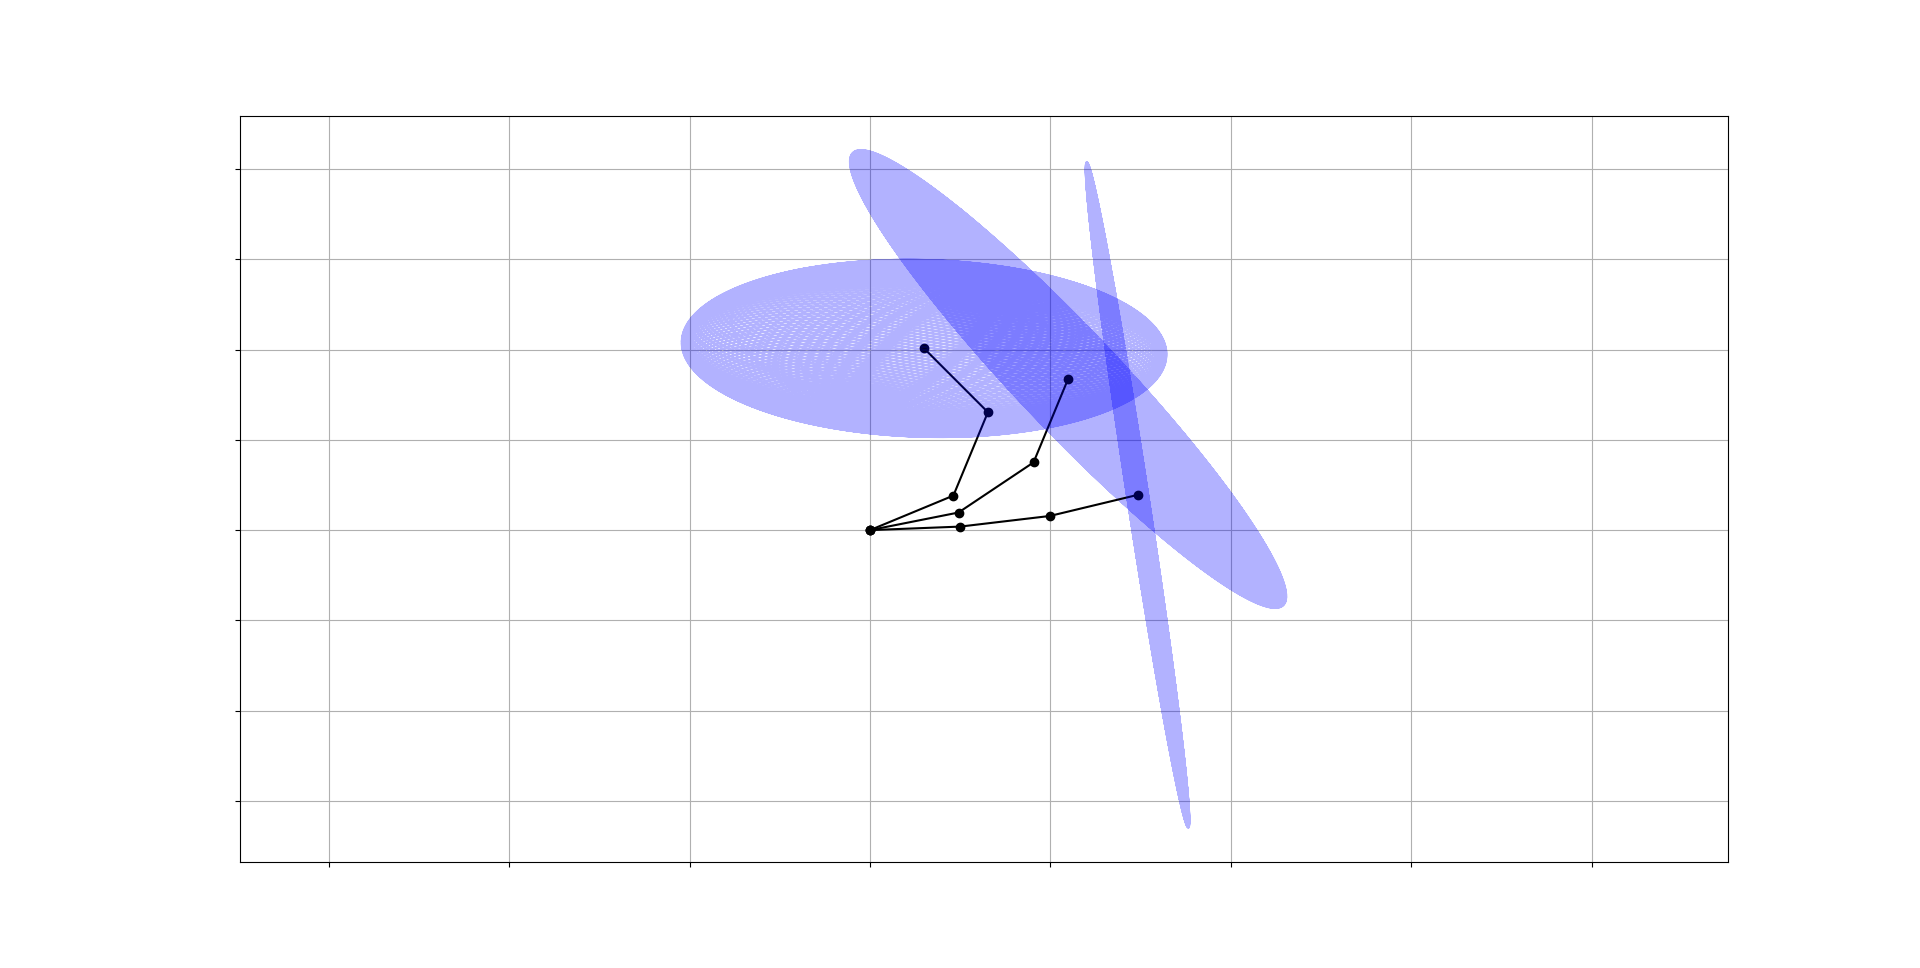
\includegraphics[width=0.9\textwidth]{Images/3r-ellipsoid.png}
    \caption{Elipsoide de manipulabilidade para diferentes configurações do manipulador planar 3R.}\label{fig:manipulability-ellipsoid}
\end{figure}

\subsection{Resolução de Redundância}

A solução geral dada pela equação (\ref{eq:pseudo-inverse}),
introduz o termo dado pelo vetor \(\dot{q_0}\) pode ser escolhido arbitrariamente. Uma
possibilidade é tomá-lo de forma a maximizar algum índice de performance \(w\),
para isso escolhendo o vetor na direção do gradiente~\cite{siciliano_robotics_2009}:

\begin{equation}\label{eq:metric-gradient}
    \dot{q_0} = k_0 {\left( \frac{\partial w(q)}{\partial q} \right)}^\top
\end{equation}

onde \(k_0 > 0\) é uma constante positiva que determina o tamanho do passo.

Uma escolha natural para o índice de performance \(w\) é a \emph{medida de
    manipulabilidade de Yoshikawa}~\cite{yoshikawa1983}:

\begin{equation}\label{eq:yoshikawa}
    w(q) = \sqrt{\det(J(q){J(q)}^\top)}
\end{equation}

onde vale ressaltar que é equivalente àquela definida na a equação
(\ref{eq:manipulability}) uma vez que se \(\lambda_i\) são os autovalores de
\(J J^\top\) então \(\sigma_i = \sqrt{\lambda_i}\).

Uma alternativa ao cálculo da \ref{eq:yoshikawa} é utilizar uma métrica mais simples como a
\emph{distância para os limites mecânicos das juntas} dada por:

\begin{equation}
    w(q) = -\frac{1}{2n} \sum_{i=1}^{n}{{\left(\frac{q_i - \bar{q_i}}{q_{iM} - q_{im}}\right)}^2}
\end{equation}

Ao maximar tal índice, espera-se que o manipulador mantenha-se próximo ao ponto
central de atuação de cada junta, evitando assim configurações singulares no
limite do espaço de trabalho. Além disso, o vetor gradiente pode ser calculado
de maneira analítica onde cada coordenada é dada por:

\begin{equation}\label{eq:joint-distance-grad}
    \frac{\partial w(q)}{\partial q_i} = -\frac{1}{n} \frac{q_i - \bar{q_i}}{{(q_{iM} - q_{im})}^2}
\end{equation}

Outro ponto a salientar é que a escolha do tamanho do passo \(k_0\) é crucial
para a performance do algoritmo~\cite{siciliano_springer_2008}. Se \(k_0\) 
for muito pequeno o processo de otimização pode se tornar muito lento, enquanto 
que se \(k_0\) for muito grande isso pode a uma diminuição ou até
 mesmo não convergência do valor de \(w\) devido a oscilações em torno do ponto 
 de máximo local.

O próximo capítulo, aplica os conceitos apresentados até agora na
concepção de um ambiente simulado para um manipulador redundante com cinco
graus de liberdade. O objetivo principal será a execução de trajetórias
cartesianas no espaço de trabalho \(\mathcal{T} \in \text{SE}(3)\) que levam
apenas em consideração a posição do efetuador e com isso explorar a resolução
de redundância para otimizar diferentes índices relacionados a configuração do
manipulador durante a execução da trajetória.
